\documentclass{article}

\usepackage[portuguese]{babel}
\usepackage[utf8]{inputenc}
\usepackage{graphicx}


\title{Relatório BDAD - Entrega 2}
\date{31-3-2015}
\author{João Cabral, up20130495\\
	   João Mota, up201303462\\
	   Luís Morais, up200800621\\}

\begin{document}

\maketitle
\pagenumbering{gobble}
\newpage
\pagenumbering{arabic}
\renewcommand*\contentsname{Sumário}
\tableofcontents
\newpage
\section{Introdução}
No âmbito da unidade curricular de Bases de Dados foi solicitada a elaboração de um
trabalho prático de tema livre. O presente relatório constitui a terceira das três entregas
previstas nas regras desse trabalho, focando-se na síntese de queries pertinentes à 
base de dados desenvolvida nas entregas anteriores, bem como
à concepção de triggers que permitam maior segurança na base de dados acima referida.


\section{Descrição de Contexto}
Pretende-se com este trabalho elaborar uma base de dados que permita guardar
informação acerca do funcionamento de um instituto prisional. Neste instituto prisional é
necessário guardar informação sobre tanto prisioneiros como funcionários.
Acerca de prisioneiros é necessário saber o nome, número de prisioneiro, data de entrada
e a data em que sairá da instituição prisional.

É ainda associado a cada prisioneiro:
\begin{itemize}
\item Uma lista de penas, cada pena contendo uma duração, data de sentença e um motivo;
\item Uma cela, generalização de local, à qual é atribuída um número de cela;
\item Um registo de todos os incidentes em que o prisioneiro esteve envolvido ao longo da sua estadia no estabelecimento prisional, cada incidente com uma descrição e uma data e associado a um local, um ou mais funcionários relatores e ainda a uma penalização. Cada penalização pode ainda ser associada a uma pena;
\item Uma lista de recompensas por bom comportamento, que se resumem a tempo adicional de recreio, sobre o qual se guarda a duração, ou o direito a objetos pessoais, sobre os quais se guarda uma descrição.
\end{itemize}
Sobre cada funcionário é necessário guardar o nome e o cargo que desempenha na prisão, bem como a hora de início e a hora de fim do trabalho e ainda o seu vencimento.
\newpage

\section{Descrição dos Conceitos}
\begin{description}
\item[Pessoa] Superclasse que engloba os atributos comuns entre prisioneiros e funcionários.
\item[Prisioneiro] Subclasse de Pessoa que guarda os dados dos prisioneiros: Data de inicio e
data de fim da pena que tem de cumprir.
\item[Funcionário] Subclasse de Pessoa que guarda os dados dos funcionários
\item[Incidente] Guarda os incidentes em que um ou vários prisioneiros se envolvem, bem como o local onde aconteceram e o/os funcionários que os testemunharam. Pode gerar uma penalização para o prisioneiro.
\item[Pena] Guarda os dados da pena de cada prisioneiro: duração e a descrição da pena
\item[Penalização] Guarda a descrição da penalização de um incidente. As penalizações podem ou
não aumentar a duração da pena.
\item[Recompensa] Superclasse que engloba os tipos de recompensa que os prisioneiros podem receber por bom comportamento.
\item[Tempo de recreio] Subclasse de Recompensa onde é guardado a duração de tempo de recreio atribuído a um prisioneiro por bom comportamento.
\item[Objeto pessoal] Subclasse de Recompensa onde é guardado o objecto cedido a um prisioneiro por bom comportamento.
\item[Local] Espaço físico da prisão podendo ser dedicado a vários propósitos
\item[Cela] Subclasse de Local, estando associada a um número de cela. Pode estar vazia ou conter um ou mais prisioneiros.
\end{description}
\newpage
\section{Esquema Conceptual}
\begin{center}
  \makebox[\textwidth]{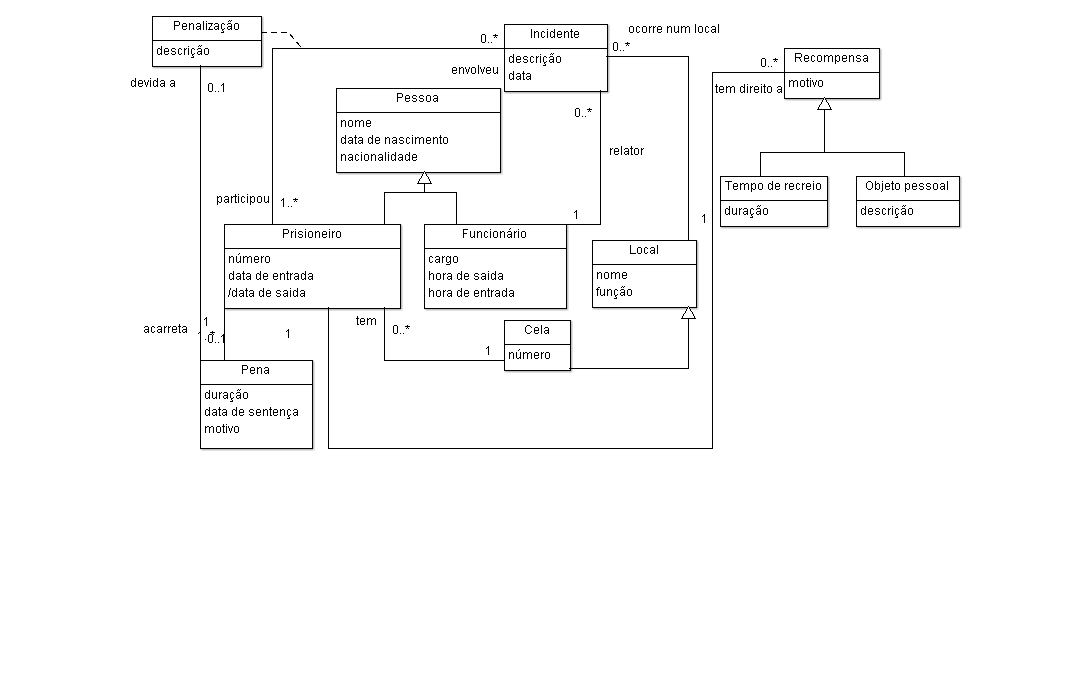
\includegraphics[width=\paperwidth]{losdiagramas.png}}
\end{center}
\newpage
\section{Esquema Relacional}
Pessoa(\underline{idPessoa}, nome, dataNascimento, nacionalidade)\\
Prisioneiro(\underline{ idPessoa} $\rightarrow$ Pessoa, data de entrada, data de saída, cela $\rightarrow$ Cela)\\
Funcionário(\underline{idPessoa} $\rightarrow$ Pessoa, cargo, hora de entrada, hora de saída, dataContratação, vencimento)\\
Tempo de Recreio(\underline{idRecompensa $\rightarrow$ Recompensa}, horaInicío, horaFim )\\
Objeto Pessoal(\underline{idRecompensa $\rightarrow$ Recompensa}, descrição)\\
Local(\underline{idLocal},nome, função)\\
Cela(\underline{número}, idLocal $\rightarrow$ local)\\
Pena(\underline{idPena}, data de sentença, motivo, idPessoa $\rightarrow$ Prisioneiro)\\
Incidente(\underline{idIncidente}, descrição, data, idLocal $\rightarrow$ Local, relator $\rightarrow$ Funcionário )\\
PrisioneiroIncidente(\underline{prisioneiro $\rightarrow$ Prisioneiro}, \underline{incidente $\rightarrow$ Incidente})\\
Penalização(\underline{idPessoa}$\rightarrow$ Prisioneiro, \underline{idIncidente} $\rightarrow$ Incidente, {idPena}$\rightarrow$ Pena, descrição)\\
Recompensa(\underline{idRecompensa}, motivo, idPrisioneiro $\rightarrow$ Prisioneiro)\\








	
\end{document}
